\task{ Плот и моторная лодка одновременно начинают движение из пункта
  \textbf{A}. Лодка проходит путь $AB=S_1$ за время $t$ и возвращается
  обратно. На расстоянии $BC=S_2$ лодка встречает плот
  (см. рис.). Найти скорость течения и собственную скорость
  лодки. Решите эту задачу в системе отсчёта а) земли; б) лодки; в)
  плота.
  \begin{center}
    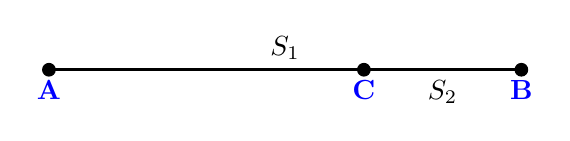
\begin{tikzpicture}
      \draw[very thick] (0,0) node[below,blue] {\textbf{A}} --
      (4,0) node[below,blue] {\textbf{C}} -- (6,0) node[below,blue]
      {\textbf{B}} node[below,midway] {$S_2$};
      \draw (0,0) -- (6,0) node[above,midway] {$S_1$};
      \draw[fill=black] (0,0) circle (0.08cm);
      \draw[fill=black] (4,0) circle (0.08cm);
      \draw[fill=black] (6,0) circle (0.08cm);        
    \end{tikzpicture}
  \end{center}
}
% Шапиро-Бодик-1, стр. 11
% ccpe-2016-2017-8